\chapter{Introduction}
Snow in Idaho serves a critical role not only for recreationists but for the state economy. A majority of irrigated agriculture in Idaho relies on surface water managed by a series of canals and reservoir systems. A majority of this water comes as snow during the winter months and is then stored in reservoirs for use during the growing season. Because of this, water managers in Idaho are actively looking for ways to better predict snowmelt runoff. Also, snow and snowmelt can have significant impacts on infrastructure and transportation throughout the state. By looking at specific snowpack characteristics, it's possible to gain insight into conditions leading to avalanche hazards, floods caused by rain on snow events, and significant runoff.  

The physical properties of snow play an essential role in avalanche prediction. Under the right conditions, temperature gradients within a snowpack drive vapor migration. As vapor migrates through and out of the snowpack, it changes the snow's microstructure and can lead to a substantial water loss of 15\% - 20\% (\cite{hood_williams_cline_1999, marks_dozier_1992, kattelmann_elder_1991}). Continuous monitoring of snowpack temperature gradients is valuable for avalanche forecasting because the development of weak, faceted layers, such as depth hoar, depends on a temperature gradient. This process is temperature-gradient, or constructive metamorphism, and the rate in which it occurs depends on several different factors; such as the initial snow characteristics, magnitude and duration of temperature gradients, vapor barriers caused by ice layers, and the snowpack's cold content (\cite{sommerfeld_1970, colbeck1983theory}). Although this is a continuous process that occurs at a wide range of temperature gradients, the critical gradient to produce faceted forms in alpine snow is about 10\textdegree C/m (\cite{mcclung_schaerer_2009}). When temperature gradients are less than critical, the snow undergoes destructive metamorphism and water molecules move mainly by vapor diffusion to new positions that decrease the surface free energy (Sommerfield). Thus, destructive metamorphism is controlled by surface convexities, and leads to rounding and bonds forming between individual snow grains. Both time and temperature are significant factors in determining the stage of metamorphism. If the snow is very cold, it will change slowly; and if it's close to the freezing point, it can change rapidly. In the case of depth hoar, if the critical temperature gradient no longer persists, the snow will undergo equi-temperature metamorphism, which breaks down many of its facets (Sommerfield).

It is important to consider the thermal conductivity of snow. The thermal properties of snow vary with density, microstructure, and temperature (\cite{arenson2015physical}). The thermal conductivity of snow ranges from 0.04 to 1 W/m/K over the density range of 100 - 550 $kg/m^3$. Although thermal conductivity varies primarily with density, variations in microstructure and crystal anisotropic orientation can affect it by a factor of two. Figure \ref{fig:ThermalConductivity} shows how effective thermal conductivity increases with snow density. Thermal conductivity variations near ice layers can induce large temperature gradients that lead to faceted, weak layer formation, and is a significant cause of avalanches.  (\cite{arenson2015physical}). 

 \begin{figure}[!t]
    \centering
    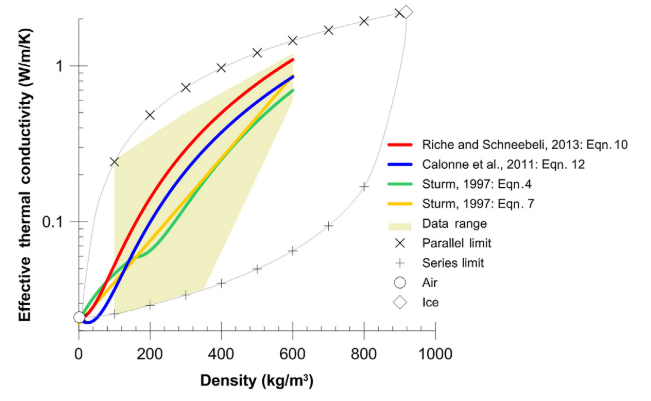
\includegraphics[width=0.8\linewidth]{figures/TempGrad/Density_Conductivity.png}
    \caption{Figure from \cite{arenson2015physical} showing the variation of thermal conductivity with density, the range of data in the literature summarized by \cite{sturm1997thermal}, and several proposed models.}
    \label{fig:ThermalConductivity}
 \end{figure}

At Banner Summit in Idaho, a significant concern for avalanche forecasters is in the development of depth hoar. Depth hoar is large-grained, faceted, cup-shaped crystals near the ground and forms because of large temperature gradients within the snowpack (\cite{akitaya1974}). This phenomenon most commonly happens in the early season because the snowpack is shallow, and there isn't much snow insulating the lowest layers from the cold atmosphere. In central Idaho, the geothermal heat flux keeps the snow-ground interface temperature very close to 0 \textdegree C (Figure \ref{fig:GroundTemp}). This condition combined with a shallow snowpack and cold air temperatures, leads to the large sustained temperature gradients in the early season. The duration and magnitude of critical temperature gradients in the lower snowpack is not well understood. 

 \begin{figure}[!t]
    \centering
    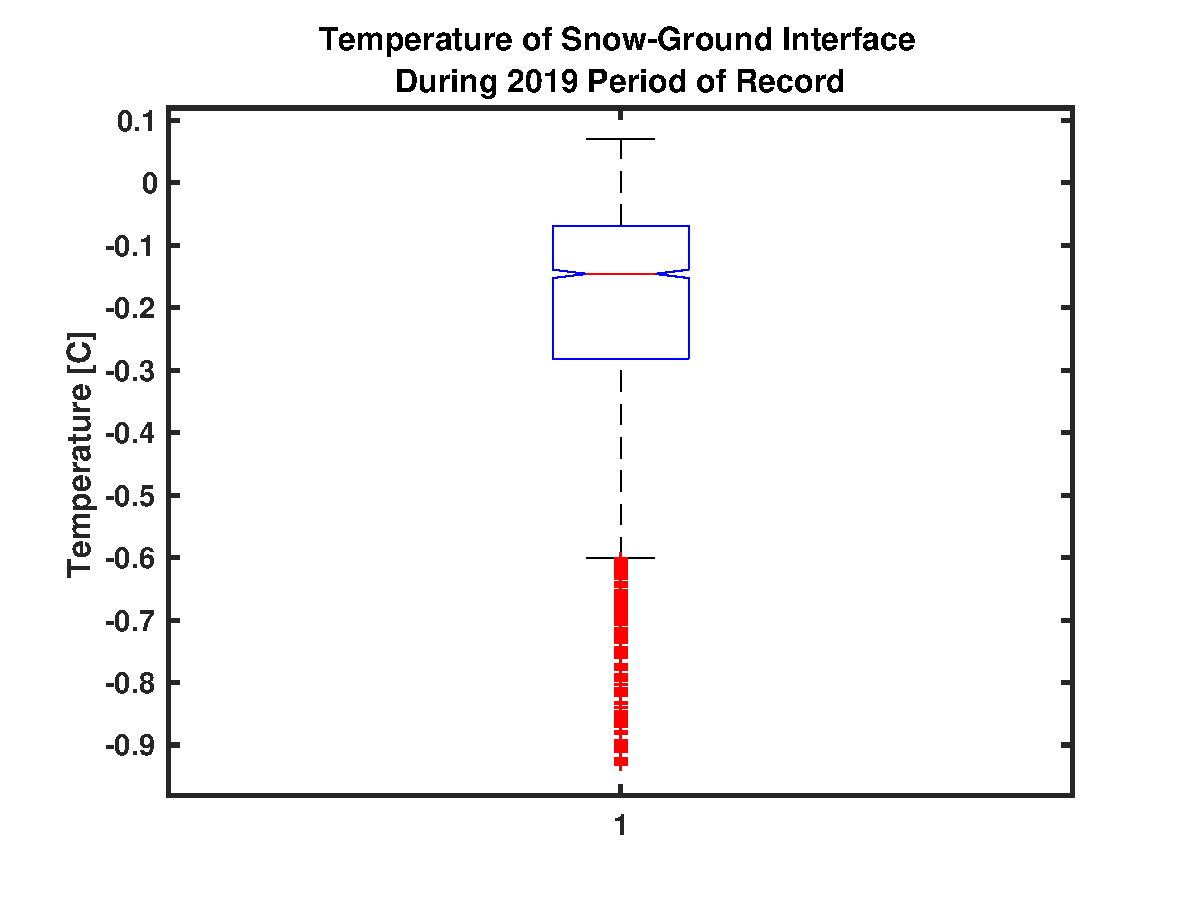
\includegraphics[width=0.8\linewidth]{figures/TempGrad/GroundTemp.eps}
    \caption{Temperature of snow-ground interface during the 2019 period of record. The ground remains at, or near the freezing point for the whole season}
    \label{fig:GroundTemp}
 \end{figure}

Dry-snow avalanches are primarily a concern in the early to mid-winter season. As spring approaches, a snowpack temperature profile provides insight into the snowmelt process. There are are three primary phases a snowpack must go through to have considerable melt and runoff; warming, ripening, and output (\cite{dingman2015}). Any energy absorbed by the sub-freezing snowpack during the warming phase raises its average temperature until it reaches isothermal conditions at 0\textdegree C (\cite{dingman2015}). This energy required to warm a snowpack to isothermal conditions is known as the cold content (Q\textsubscript{cc}) (\cite{dingman2015}), and can be calculated directly from the temperature profile:

\begin{equation}
Q\textsubscript{cc} = -c\textsubscript{i}*\rho\textsubscript{w}*h\textsubscript{m}*(T\textsubscript{s}-T\textsubscript{m)}
\end{equation}

Where c\textsubscript{i} is the heat capacity of ice, T\textsubscript{s} is the average temperature of the snowpack, T\textsubscript{m} is the melting point of ice, $\rho\textsubscript{w}$ is the desnity of water, and h\textsubscript{m} is the snow water equivelence (SWE). 

Once the snowpack is isothermal, it enters the ripening phase where absorbed energy melts snow, but the meltwater is retained in the snowpack by surface tension forces (\cite{dingman2015}). After the snowpack reaches its water holding capacity and it is "ripe," then it is in the output phase where further absorption of energy produces water output (\cite{dingman2015}). Because isothermal conditions mark the beginning of the ripening phase, it may be possible to predict snowmelt runoff timing more accurately by measuring the snowpack's temperature profile continuously.

Snow is a prime example of the observer effect; the mere observation of a phenomena within the snowpack inevitably changes the phenomena. The current method for measuring the temperature profile of a snowpack is a time consuming, destructive process that is not automated. The present method is destructive because it requires someone to dig a snow pit and manually measure the snow temperature by inserting probes at equal depth intervals. Not only does this disturb the snow profile and change its characteristics, but it’s a snapshot in time, while snow temperature conditions change on an hourly time scale in the upper part of the snowpack, and on a weekly time scale at depth.

Here, we present a continuous snowpack temperature monitoring system, the Banner Summit Thermocouple Array (BSTA) along with methods for analyzing the in the context of temperature gradient metamorphism and melt. Results suggest this instrument is successful at measuring the temperature profile of a snowpack with a temperature accuracy of \isostd \ (Figure \ref{fig:Iso_Temp_Hist}) and an uncertainty in temperature gradient estimates of \gradstd \ (Figure \ref{fig:MC_Grad}). This data further develops our understanding of temperature gradient metamorphism in snow, and it provides insight into snowpack processes that lead to significant snowmelt.

It is important to note that current technology can only measure a snowpack temperature profile at a single point in space, rather than the basin scale. Although snowpack conditions can vary widely at the basin scale, the BSTA serves as a valuable tool because it may be possible to build statistical relationships between this site and things like nearby stream gauges, or avalanche starting zones. The ability to conduct statistical analysis for avalanche hazards and snowmelt runoff will only come with a continuous record from the BSTA at Banner Summit.  